

\documentclass[11pt,a4paper,titlepage,oneside]{article}

\usepackage[most]{tcolorbox}
\usepackage{geometry}
\usepackage{svg}

\usepackage{hyperref} %links
\usepackage{xurl}

\usepackage[document]{ragged2e} %floating text
\usepackage{helvet} %font
\usepackage{tocloft} % dots in table of contents sections

\usepackage{lipsum, multicol}
\usepackage{fancyhdr}
\usepackage{listings}


% citaitons
\usepackage{natbib}

% hypthenationrules
\usepackage[T1]{fontenc}



%redefine the entire fucking bib environment so we dont have the horisontal spacing
% this was generated entirely by chatgpt

\makeatletter
\renewenvironment{thebibliography}[1]
  {\section{Lähteet}%
   \@mkboth{\MakeUppercase{\refname}}{\MakeUppercase{\refname}}%
   \list{\@biblabel{\@arabic\c@enumiv}}%
        {\settowidth\labelwidth{\@biblabel{#1}}%
         \leftmargin\labelwidth
         \advance\leftmargin\labelsep
         \setlength\itemindent{-\labelwidth}
         \setlength\itemsep{10pt} % Change this value to adjust the space between items
         \@openbib@code
         \usecounter{enumiv}%
         \let\p@enumiv\@empty
         \renewcommand\theenumiv{\@arabic\c@enumiv}}%
   \sloppy
   \clubpenalty4000
   \@clubpenalty \clubpenalty
   \widowpenalty4000%
   \sfcode`\.\@m}
  {\def\@noitemerr
    {\@latex@warning{Empty `thebibliography' environment}}%
   \endlist}
\makeatother





%this is such a shitshow lmao

\hypersetup{
    colorlinks=false,
    citecolor=black,
    filecolor=black,
    linkcolor=black,
    linkbordercolor=1 1 1,
    citebordercolor=1 1 1,
    pdfborderstyle={/S/U/W 1},
    urlbordercolor=0 0 1,
    urlcolor=blue
}
\urlstyle{same}



\geometry{
    a4paper,
    left=3cm,
    right=2.5cm,
    top=3cm,
    bottom=2.5cm
}

%remove random margin on side ? idk what happend
%\setlength{\oddsidemargin}{0pt}



%custom reusable colorbox rules
\newtcolorbox{simplebox}{colback=white, sharp corners, boxrule=1pt }


\renewcommand{\contentsname}{Sisällys} % override Contents => Sisallys on table of contents

\renewcommand{\familydefault}{\sfdefault} % set font

\renewcommand{\cftsecleader}{\cftdotfill{\cftdotsep}} % dots for sections

\renewcommand{\bibsection}{\section{Lähteet}}



\def\filename{src/oppari.tex}



\def\testmode{1}






\newcommand\wordcount{
    \immediate\write18{texcount -sub=section \filename{} -inc  | grep Section | sed -e 's/+.*//' | sed -n \thesection p > 'count.txt'}
(\input{count.txt}words)}


\newcommand{\inputf}[1]{\def\filename{#1}\input{#1}}


\newcommand\filewcount{
    \immediate\write18{texcount -1 -sum \filename{} > count.txt }
    \input{count.txt} words }


% jos on testi definetty niin tee 
\newcommand{\istest}[2]{\ifx\testmode\undefined #2 \else #1 \fi}


% testi section näyttää word countin siltä sectionilta jos ei testi niin sitten näytä vain normaali section
\newcommand{\tsection}[2]{\istest{#1{#2\\} \wordcount \\ \medskip }{#1*{#2}}}


\newcommand{\pagesection}[1]{\istest{\section{#1}  }{\section*{#1}}}
\newcommand{\pagesubsection}[1]{\istest{\subsection{#1}  }{\subsection*{#1}}}


% adds page with everything
\newcommand{\addPage}[2]{
    \def\filename{#1}
    \pagesection{#2}
    \istest{ \filewcount \medskip }{}
    \input{#1}
}



% OPPARI SPESIFIC

\newcommand{\addPageOp}[2]{
    \def\filename{#1}
    \pagesubsection{#2}
    \istest{ \filewcount \medskip }{}
    \input{#1}
}

%lab citation style
\newcommand{\labcite}[1]{\setcitestyle{aysep={},open={(},close={.)}}\citep{#1}{}}

%lab citation style
\newcommand{\labciteend}[1]{\setcitestyle{aysep={},open={(},close={).}}\citep{#1}{}}

\newcommand{\labimgcite}[1]{\setcitestyle{aysep={},open={(},close={)}}\citep{#1}{}}

\newcommand{\hurl}[1]{\href{#1}{{\underline{\textcolor{blue}{#1}}}}}


% counter kuville
\newcounter{imgCounter}
\setcounter{imgCounter}{0}

\newcommand{\getImgCount}{
\addtocounter{imgCounter}{1}
\theimgCounter
}


% counter kaavioille
\newcounter{chartCounter}
\setcounter{chartCounter}{0}

\newcommand{\getChartCount}{
\addtocounter{chartCounter}{1}
\thechartCounter
}



\usepackage[finnish]{babel}
















% ------------------------------ BEGIN DOCUMENT ------------------------------ %
\begin{document}

\pagestyle{empty}


%------------------------------ COVER PAGE ------------------------------ %


\includegraphics[width=5cm,height=1cm]{./src/labimg.jpg}

\vspace{86mm}
\huge
\textbf{Kehityksen seuranta}
\newline

\large

\vspace{5mm}
\textbf{Oppimispäiväkirja}
\normalsize

\vspace{90mm}

LAB-ammattikorkeakoulu \newline
\vspace{2mm}
Tieto-ja tietolikenadsfklj, Insinööri (AMK) \newline
\vspace{2mm}
2024 \newline
\vspace{2mm}
Kimi Malkamäki

\newpage




%------------------------------ FIRST PAGE OF ABSTRACT ------------------------------ %
\begin{tabular}{ | l | }

    %hack for the tiivistelmä line
    \multicolumn{1}{l}{
        \begin{minipage}{6cm}
            \hspace{1mm}
            
        \end{minipage}
        \begin{minipage}{4.25cm}
            \hspace{1mm}
        \end{minipage}
        \begin{minipage}[t][1.95cm][t]{3.62cm}
            \large
            \textbf{ Tiivistelmä }
        \end{minipage}
    }\\

    \hline
    \begin{minipage}[b]{6cm}
        tekijä(t)
        \newline
        kimi malkamäki 
    \end{minipage}%
    % 2x2
    \begin{minipage}{8.5cm}
        \begin{tabular}{ | l | c | }
            \begin{minipage}[t][1cm][t]{4.25cm}
                julkaisun laji
                \newline
                Opinnäytetyö, AMK
            \end{minipage} & %
            %
            \begin{minipage}{3.62cm}
                valmistusaika
                \newline
                2024
            \end{minipage} \\ \hline%
            %
            \begin{minipage}[t][1cm][t]{4.25cm}
                sivumäärä
                \newline 
                xx+xx
            \end{minipage}
            &  \\ \hline
        \end{tabular}
    \end{minipage}%
    % end of 2x2
      \\ \hline

    \begin{minipage}[t][2cm][t]{8cm}
    Työn nimi 
        \newline 
    ammatissa kasvaminen 
        \newline 
    oppimispäiväkirja  
    \end{minipage}\\ \hline

    \begin{minipage}[t][1.5cm][t]{10cm}
    tutkinto ja koulutusala.\newline  tietoviestintätekniikka insinööri amk  

    \end{minipage}\\ \hline

    \begin{minipage}[t][7cm][t]{5cm}
    tiivistelmä: \newline lorem ipsim
    \end{minipage}\\ \hline

    \begin{minipage}[t][2cm][t]{5cm}
    avain sanat
    \end{minipage}\\ \hline

\end{tabular}

\newpage



% ------------------------------ SECOND PAGE OF ABSTRACT ------------------------------ %

tiivistelmä








\newpage


% ------------------------------ TABLE OF CONTENTS ------------------------------ %

%keep page numbers off
\setcounter{page}{0}
\pagestyle{empty}
\pagenumbering{gobble}

\tableofcontents





\newpage



% ------------------------------- TERMISTÖ ------------------------------- %


TERMISTÖ
\bigskip

(tiedän ettei termistö kirjoiteta tällä formaatilla. tämäkin on hyvin kesken)
\bigskip
 
%this needs to be aligned cannot be like this make minipage maybe
ECMAscript = skriptaus-kieli standardi 
\bigskip

DOM = Document Object Model 
\bigskip

puu = datastruktuuri(selitä paremmin)
\bigskip

VDOM = virtual DOM
\bigskip

Transpilaatio = ohjelmointi keilen kääntäminen toiseen ohjelmointikieleen
\bigskip



\newpage





% ------------------------------- CONTENT PRELUDE COMMANDS ------------------------------- %
%enable page counting
\pagenumbering{arabic}
\clearpage
\setcounter{page}{1}

%set heaader and footer
\pagestyle{fancy}
%%
\lfoot{}
\cfoot{}
\rfoot{}
%%
\lhead{}
\chead{}
\rhead{\thepage}
%%
\renewcommand{\headrulewidth}{0pt}
\renewcommand{\footrulewidth}{0pt}
%\newcommand{\n}{\newline\vspace{20mm}}


\section{Johdanto}              % ------------------------------- JOHDANTO ------------------------------- %



% jos tulee niin sitten jotain siitä että web suunnittelu liikkuu nopeaseti ja siellä on kokoajan uusia teknologioita
%mutta pohjalta ne perustuu samoihin periaatteisiin.

% tullaanko tekemään seuranta vai jos tulee tarpeeksi tekstiä niin onko ok vaan tehdä normi oppari tästä
% jos tavoitteena olisis se uuden featuren lisääminen


% jotain siitä että teknologiat tulee ja menee  ja startupit yrittää päästä mukaan koska siinä on paljon rahaa liikenteessä
(lorem tekstiä menee uusiks)\\
teknologia ala on nopeasti liikkuva. monet teknologiat ilmestyy tyhjästä ja häviää kuin tuhka tuuleen.
Suositun tuotteen tai teknologian kehittäminen ja onnistuneesti markkinoille saanti on hyvin tuottava liikemalli, 
mutta monet ketkä yrittää epäonnistuvat.
Tämä tuo haasteita alalla työskenteleville ammattilaisille, 
sillä pitää olla kokoajan ajantasalla uusista teknologioista ja työntavoista, että voi pysyä alan mukana.
\medskip


% tätä ennen tulee jotain tekstiä itse tavoite sanotaan tiivistelmässä vissiinkin
Opinnäytetyön tavoitteena on seurata kehittymistä 13 viikon seurantajakson aikana työharjoittelussa suomalaisessa startup yrityksessö
ja tutkia henkilökohtaista kehitystä harjoituksen aikana.
%more text
\medskip


Opinnäitetyö on päiväkirjamallinen ja liitteenä on päiväkirja dokumentti, 
johon on kirjattu viikottainen tehneeni työn perusteella, päiväkirjassa kerrotaan
minkälaisten teknologoiden kanssa olin tekemisissä ja mitä opin hajroittelun aikana.
%more text
\medskip


Opinnäytetyö toteutettiin Starttaamo Oy:ssä. Starttaamo on suomalainen startup yritys, joka pyrkii ratkomaan ongelmia työergonomian kanssa.
Startupin pää tavoitteena on vähentää sairaslomia saamalla työntekijät noudattamaan, alojen ammattilaisten suunnittelemien liikunta- ja ruokavalio-ohjelmia. 
% scuffed af.. web alusta jota kehitin...  jotenkin paremmin se että olin kehittämässä sitä mukana.
Yrityksen pää myyntituote on web-alusta, jonka kehityksen mukana olin.
%
Alustan kehittämisessä sain mahdollisuuden työskennellä tuotantoympäristön kanssa.
Olin mukana suunnittelussa ja ominaisuuksien ohjelmoinnissa. sain myös kokemusta ilmeentyvien ongelmien korjaamisesta.

% suunnittelussa ja ohjelmoinnissa, sain kokemusta tuotantoympäristön ohjelmoinnista.
\medskip






\newpage
\section{Lähtötilanne}         % ------------------------------- LÄHTÖTILANNE ------------------------------- %


Ennen opinnäytetyön kirjoittamista ja seurantajakson alkamista olin opiskellut LAB ammattikorkeakoulussa XX lukukautta ja olin opinnäytetyön kirjoituksen aikana neljännen vuoden tieto- ja tietoviestintätekniikkan opiskelia.
Koulutuksen aikana olen oppinut jotain 
% jotain lorem siitä että olen oppinut koulusssa jotain

\medskip



% jotain siitä että ei ole oikeaa työ kokemusta vaikka on vahva koodauspohja
Ennen harjoituksen alkamista minulla ei ollut aijempaa työkokemusta tieto- ja tietoviestintätekniikkan alalta.
% tiedän ohjelmoinnista mutta prod on eri ympäristö
Ja vaikka minulla oli vahva teoria pohja ohjelmoinnista, jonka olin saanut opinnoistani, 
käytössä olevan tuotteen kanssa työskentely on erillaista.
\medskip







\newpage
\section{Teoria}                % ------------------------------- TEORIA ------------------------------- %



\subsection{Kehitys ympäristö / Teknologia pino}

%yleisesti tässä kappaleessa voisi olla ainakin yksi kokonainen sivullinen tekstiä
%ainakin sen verran pitäisi saada kirjoitettua




% scuffed af kun käytettyjen teknologioiden lukee kahesti päällekkäin

% vähän paremmin selitys markkinoille pääsemisenn
Startup- ja muut kasvuyritykset, jonka pää tuotteena on sovellus tai muu teknologia, hakee nopeaa ja ketterää kehitystä markkinoilla pärjäämiseen.
% kirjoita kehitys nopeus paremmin
Tämä pitää ottaa huomioon käytettyjen teknologioiden valinnassa, sillä eri teknologioilla on eri kehitysnopeus.
Pohjalla käytettyjen teknologioiden vaihtaminen on erittäin työlästä jälkikäteen,
joten päätös käytetyistä teknologioista tulee määräämään yhtiön kehityksen nopeuden.
Hidas sovelluskehitys voi haitata itse yrityksen mahdollisuuksia selvitä markkinoilla.
\medskip




Teknologia pino pohjautuu MeteorJs kehykseen. Se on suunniteltu nopeaan kehittämiseen ja käyttöönottoon.
Meteor helpottaa kommunikointia käyttöliittymän, palvelimen ja tietokannan kanssa, 
mutta silti antaen vapauden valita muut käytettävät teknologiat, eikä lukitse käyttämään valmiiksi valittuja teknologioita.
Meteor ei määritä käytettyä käyttöliittymä kirjastoa mutta se silti tukee monia suosituimpia kehyksiä ja antaa halpon integraation niihin.
Projekttin on valittu ReactJs kirjasto käyttöliittymän toteutukseen.
Reactin komponentti pohjainen rakenne tekee käyttöliittymä koodista helposti uudelleen käytettävän, nopeuttaen käyttöliittymän rakentamista. 
Myös sen sisään rakennettu reaktiivisuus tilallisilla komponenteilla tuo helpon käyttöliittymä päivityksen.
Meteorilla on hyvä integraatio ReactJs:ssän kanssa. 
Tämä on nähtävillä kun Meteor päivittää automaattisesti käyttöliittymää tietokantamuutoksien tapahduttua. 
Projektissa käytössäoleva tietokanta MongoDB on kanssa hyvin integroitu Meteoriin.
MongoDBn skeematon dokumentti rakenne, tuo helpon tavan päivittää skeemmoja tarpeiden tullen.
%jokunen lause lisää mongodbstä ennen kun seuraava kapale
\medskip



MeteorJs MongoDB ja ReactJs on pohjalla olevat teknologiat, jonka päälle projekti on rakennettu.
Yhdessä näitä kolmea teknologiaa käytten voi luoda monenlaisia nopeuta ja skaalautuvia nettisivuja pienistä projekteista suuriin.
Nämä teknologiat ovat myös suunniteltu nopeaan kehittämiseen, joka tekee niistä hyvän valinnan kasvavalle startup yritykselle.
%more
\medskip









%sitatatti order kussee
\newpage
\subsection{Meteor}                % ------------------------------- Meteor ------------------------------- %



\subsubsection{meteor yleisesti}



% https://guide.meteor.com/collections.html#mongo-collections
% meteor uses mongo. but it is not manditory





Meteor on full-stack JavaScript web-framework ja on itsessään avoimeen lähdekkoodiin perustuva, \labcite{meteor24b}
poislukien meteorin mukaan paketoimaa mongodb tietokantaa, joka toimii Server Side Public Lisenssillä.\labcite{mongodb24i}
Meteor on suunniteltu nopeaan kehittämiseen monelle laitteille ja nopeaan käyttöönottoon ja se keskittyy isomorphiseen koodiin, 
eli koodiin joka on samanlaista palvelimella kuten clientillä.\citemissing
Meteor ei määritä käytettyä front-end teknologiaa vaan sillä on integraatio moneen yleiseen frontend-framework:kiin, kuten Vue, React, Svelte tai Angular.\labcite{meteor24a}
Tämä antaa lisä joustoa Meteorille sillä se antaa mahdollisuuden monelle sovelluskehittäjälle joilla ei ole kokemusta tietystä front-end teknologiasta.



\medskip

% asio ok mut kirjota paremmin ja uusiks varm gpt on ok täs vaihees
%paremmin alku 
Meteor on fullstack, joten kun sen käynnistää se käynnistää samalla palvelimen ja clientin.
Tiedostorakenteessa on erityks kansioita kuten server ja client jota käyttäen Meteor tietää mitä koodia pitää ladata clientille ja mitä palvelimelle.
%more text




\medskip

    
% https://www.meteor.com/
% viitattu 28.5

% tukee sana pitää vaihtaa sillä me käytetään sitä itemeissä
Lisäksi Meteor tukee monta ominaisuutta kuten. \labcite{meteor24a}
\begin{itemize}
    \item Tukee monta Front-end kirjastoa ja frameworkkkia
    \item Tukee Typescriptiä
    \item Sisään rakennettu käyttäjä systeemi
    \item Toimii monella laitteella
    \item Helppo ja nopea käyttöönottaa 
\end{itemize}
\medskip


Meteor paketoi mukaansa käyttäjä paketin jota käyttäen kehitäjä voi nopeasti luoda authentikaatio järjestelmän.
Käyttäjä paketti antaa helpon integraation muiden kirjautumis palvelujen kanssa kuten facebook, github, google ym. \labcite{meteor24c}
Käyttäjä paketti on myös integroitu muihin Meteorin ominaisuuksiin kuten metodeihin.
%maby more txt



\subsubsection{Meteor metodit}

% kirjoita tämä oikeella oppari tyylillä. idk tuntuu vähän väärältä tässä


% kappale rpc. mikä on ja miten eroaa restful

%enemmän yleis selostusta rps ja restful mikä on ero hyvät ja huonot puolet

Meteor käyttää RPC (eng Remote procedure call) rajapintaa \labcite{meteor24a} perinteisen RESTful rajapinnan sijasta. % ne on asynkroonisia callback funktiolla
Tämä antaa mahdollisuuden clientille kutsua funktioita palvelimella Meteorin kautta.
% joku selitys että metodi on rpc
Meteorin RPC rajapinnat ovat Meteor metodit.
%jotain muuta loremia ennen ku mennään metodit käytännössä vaiheeseen
\medskip


Metodit määritetään ja suoritetaan palvelimella kuten kuvassa \nextImageCount.
%selitä isomorpinen paremmin tässä kontekstissa
%koodi on metodi kutsu on samaa clientillä ja palvelimella joten metodeja voi helpommin uudelleen käyttää 
Metodit tekee myös koodista yksinkertaisemman sillä clientin ei tarvitse tehdä GET tai POST requesteja palvelimelle, kun halutaan palvelimen tehdä jotain. 
Ja koska metodi kutsu on myös isomorphinen, metodeja on helppo uudelleen käyttää palvelimella.
% tutki onko tämä oikea selitys
Metodi funktion "this"{} ominaisuus saa kutsujan kontekstin. 
Tässä kontekstissa voi nähdä esimerkiksi onko kutsuja kirjautunut sisään, tai onko kutsujalla oikeat oikeudet kutsua metodia, 
helpottaen turvallisuuden lisäämista rajapintaan.
\bigskip

% jos tarvitaan lisää niin kuva metodista ja sen kutsumisesta
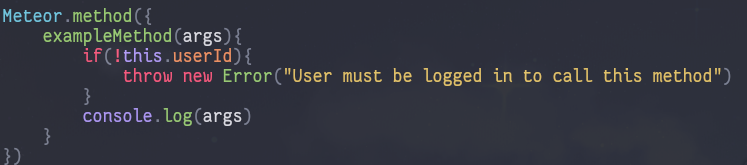
\includegraphics[width=15cm]{src/public/methodexample.png}\\
Kuva \getImgCount {}. Meteor metodin määritelmä
\medskip

% tutki onko tämä accurate selitys asiasta
Kuvassa on meteor metodin määritelmä. "exampleMethod"{} metodi katsoo, onko kutsujalla käyttäjä tunnusta, näin voimme tietää onko kutsuja kirjautunut sisään,
jos käyttäjä ei ole kirjautunut sisään heitämme error viestin, joka välitetään kutsujalle.
Jos käyttäjä on kirjautunut sisään tulostetaan argumentit. 

\medskip




\subsubsection{Meteor ecosysteemi}

% jotain package management
%https://www.linkedin.com/pulse/build-apps-isomorphic-ecosystem-meteorjs-pranav-shah
% 18.6 

%more about athmosphere
%https://guide.meteor.com/using-atmosphere-packages
% 18.6 


% yhdistä lauseet paremmin, elä aloita jokainen lause Meteor sanalla
Meteor ylläpitää omaa paketointi ecosysteemiään.
Meteor paketit ovat isomorphisia, eli ne toimivat palvelimella ja clientillä.\labcite{pranav17}{}
Meteorilla on ensimmäisen osapuolen paketteja, joita itse meteor tiimi ylläpitää ja kolmannen osapuolen paketteja,
% selitä athmosphere paremmin
joita yhteisö ylläpitää. Nämä kolmannen osapuolen paketit voi ladata Meteorin paketti palvelimelle Athmosphere:lle.
%more text



\medskip

%ihansama miten tämä kirjoitetaan se kuulostaa mainostuksetla 
% mutta kyllä tästä pitäisi jokunen lauseke saada ulos

Galaxy on meteorin deploy service millä voi helposti deploy meteor sovelluksen pilveen.







\newpage
\addPageOp{./src/op/react.tex}{React}% ------------------------------- REACT ------------------------------- %






\newpage
\addPageOp{./src/op/mongo.tex}{MongoDB}        % ------------------------------- MONGODB ------------------------------- %











\newpage
\subsection{Responsiiviset käyttöliittymät}

\subsubsection{Responsiivisten käyttöliittymien suunnittelun periaatteet}

WORK IN PROGRESS LOREM FOR RESPONSIIVINEN
\medskip


% kirjoita eritavalla ettei oo copypasta
Responsiivinen verkkosuunnittelu on lähestymistapa verkkosivustojen rakentamiseen, jolla varmistetaan niiden optimaalinen ulkoasu ja toimivuus eri laitteilla ja näytön koossa.
Käyttämällä responsiivisia verkkosuunnittelua verkkosivustot voivat tarjota yhdenmukaisen käyttökokemuksen eri laitteilla.

idea on tehdä verkkosivu jota voi käyttää eri laitteilla, jolla on eri näytönkoot
\medskip


% uudelleen kirjoita jotankin että sama asia mutta ei copypasta kuitenkaan päiväkirjasta
Web-käyttöliittymissä elementtien koot voivat olla absoluuttiset tai suhteelliset niiden ylempään elementtiin verrattuna. Absoluuttiset arvot tarkoittavat, että elementti olisi aina tietyn kokoinen pikseleissä. 
Tämä voi luoda tilanteita, jossa pienempikokoisemman näytöllä joku elementti on liian iso, tai ei sovi enää käyttöliittymään, joten absoluuttisia ei voi käyttää responsiivisessa käyttöliitymässä.
% asiakielellä. eivät kuitenkaan ei kuulosta oikeelta jutulta
Relatiiviset elementtikoot eivät kuitenkaan ratkaise kaikkia ongelmia. Mobiili- ja työpöytälaitteiden kuvasuhteet eroavat. Käyttöliittymän pitää olla erilainen jos pituutta on enemmän, kun leveyttä. 
Ja, koska työpöytälaitteita käytetään hiirellä, joka antaa tarkan osoittimen käyttäjälle, toisin kuin mobiilissa, jota käytetään sormilla. 
Pitää ottaa huomioon linkkien, nappien ja kuvakkeiden koko, jotta itse sovelluksen käyttäminen olisi huoletonta.\medskip
\medskip




\subsubsection{Css Mediaquery}

lorem ipsum

lorem ipsum






\newpage
\subsection{Web sivustojen kääntäminen}

% sana lokalisaatio pitäisi vaihtaa translaatioksi
% sillä me emme tehnyt mitään oikeaa lokalisaatiota


%link tree
% https://www.linkedin.com/pulse/website-translation-how-to-guide-louise-souter


% people prefer content in their lenguage
%https://csa-research.com/Featured-Content/For-Global-Enterprises/Global-Growth/CRWB-Series/CRWB-B2C#10Facts
% 11.6


%kääntäminen yleisesti ja miksi sen tekisi. ja jotain itse lokalisaatiosta

Kielimuuri on iso ongelma tuotteiden ja nettisivujen laajentamisessa uusille markkinoille.
% uusiks
csa rechearching väittää että 65\% käyttäjistä suosisi sisältöä heidän kielellä.
\medskip





%https://www.transifex.com/blog/2024/website-translation-methods/
%11.6 

On monta eri menetelmää sivustojen kääntämiseen, 
ja koska monet kielet on hyvin erillaisia voi konteksti ja nuanssi hävitä jos kääntää vain sana sana sanaan.
Monet lausahdukset ja sanonnat ei voi kääntää suoraan kielestä toiseen ilman että menettää sen alkuperäisen tarkoituksen.
esimerkiksi (joku esimerkki sanonnasta joka ei toimi jos sen kääntää englanniksi).
\medskip


%add more words to this
Käännös teksin luonnin voi yleisesti tehdä kahdellla tavalla. Ihmis käännös tai tekoälykäännös.
Ihmis käännöksellä voi olla hyvä tarkkuus ja lopputulos tulee kuulostamaan luonnolliselta.
tekoaly käännös on tosi nopea, mutta ei vielä ole tarpeeksi tarkka kaikkiin käyttötarkoituksiin.
\medskip




%https://www.motionpoint.com/platform/what-are-the-best-technologies-for-website-translation/
% 11.6


On eritapoja toteuttaa käännösten tekeminen web alustoilla. Monet suuret sivustot kutem amazon \citemissing{} 
hostaa monta eri versiota niiden nettisivuista.
legit hard kopio nettisivusta joka on kirjoitettu eri kielellä. Tämä on hyvin kallis ja aikaavievä.

Tekstin Hot swappaaminen. Käytetään yhtä sivua mutta teksti vaihtuu alta kun vahdetaan kieli. \citemissing{}
käytetään jotain keskitettyä kielipankkia johon kaikki käännökset on tallennettuna.
\medskip


Hot swappaamisessa...\\
Kovakoodatut tekstit sivuilta vaihdetaan käännösfunktiokutsuihin.
Funktio etsii käännöstiedostosta oikeat sanat tai lauseet ja asettaa ne alkuperäisen tekstin tilalle. 
Käännöstiedost on avain-arvo. %jotain tähän vielä
% asiakielellä uusiks
Avain on valmiiksi päätelty merkkijono ja arvo on itse käännös. 
Kun haluttu kieli vaihdetaan kirjasto vaihtaa käännöstiedoston toiseen tiedostoon jolla on samat avaimet. 
Arvot vain vaihtuvat uuden kielen tekstiksi.\citemissing
\medskip












\newpage
% mahdollissesti toteutus title pois että saa yhden lisää subsectiionin muuten tää on vähän liikaa alalukuja



% mahdollissesti toinen sectio missä puhun starttaamolla työskentelystä



\section{Käännösten toteutus}

\subsection{wip title tehtävä}
Sovelluksen sivut on kovakoodattu suomeksi. ja ne pitäisi pitäisi pystyä kääntämään.
\medskip


\subsection{Käytetty teknologia}
Meteorin kanssa yhteensopiva i18n kirjastoa käyttäen käännöksien luonti ei ole monimutkaista.
Kaikkien julkisesti olevien teksien etsiminen ja vaihtaminen i18n käännös funktio kutsuihin.
Käännös tiedoston luominen ja käännöksien laittaminen.
\medskip
\bigskip


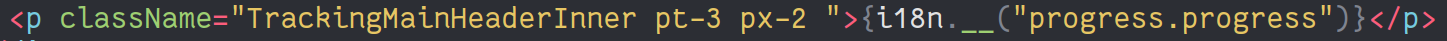
\includegraphics[width = 15cm]{src/public/oppar/translationcall.png}\\
Kuva \getImgCount. {} i18n käännösfunktiokutsu (ehkä uusi kuva)
\medskip

kuvassa luodaan HTML paragraafi elementti jossa kutsutaan käännösfunktiota. funktio hakee käännöstiedoston progress sivulta progress arvon.
\bigskip


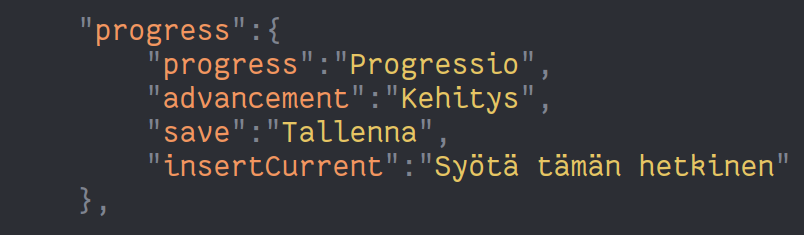
\includegraphics[width = 15cm]{src/public/oppar/translationfile.png}\\
Kuva \getImgCount. {} progressiosivun käännökset suomenkieliseltä käännöstiedostosta(ehkä uusi kuva)
\medskip

kuvassa progressio sivun käännökset. käännös tiedoston on json formaatissa joten sivut ovat omia objekteja. 
niiden ominaisuudet ovat avaimia mitä käytetään kun haetaan käännöksiä ja arvot ovat julkinen teksi.
Kuvassa \nextImageCount {} On Sama kohta käännöstiedostosta mutta englannin kielisestä
\medskip
\bigskip


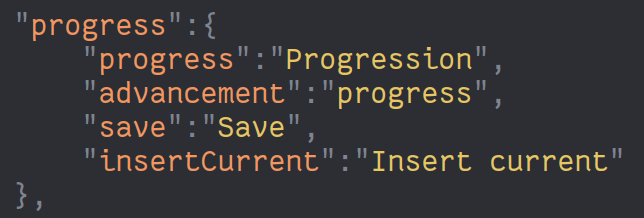
\includegraphics[width = 15cm]{src/public/oppar/translationfileEng.png}\\
Kuva \getImgCount {}. progressiosivun käännökset englanninkielisestä käännöstiedostosta(ehkä uusi kuva)
\medskip




% tämän kappaleen voisi poistaa. 
% lisätä tää toiseen kappaleeseen tai sitten poistaa kokonaan
\subsection{käyttöliittymä kielenvaihamiselle}

%lisäsin sivulle, tosin kun sivulle on lisätty
Sivulle on myös lisätty laskuvalikko kielen vaihtamiselle. 
Kielet kuvataan lippuina laskuvalikossa.
Liput toimivat nopeina visuaalisina vihjeinä, jotka auttavat käyttäjiä tunnistamaan haluamansa kielen.
kuvassa \nextImageCount.



\bigskip

\includegraphics[]{src/public/locale_laskuvalikko.png}\\
Kuva \getImgCount {}. Kielen vaihto laskuvalikko


\subsection{wip title kaksi}
Sovelluksen kaikki julkisesti oleva teksi on siirretty käännös tiedostoihin. 
Tämä luo keskitetyn sijainnin josta voi helposti etsiä ja korjata kirjoitus virheitä ja lisäämään uusia lauseita ja sanoja.
uuden kielen lisääminen vaatii uuden käännöstiedoston luomisen ja käännös arvojen asettelun tiedostoon.
\medskip

% saadaanko jotain lisää kirjoitettua ns "yhteenvetoon"










\newpage
\addPage{src/op/feature.tex}{Uuden ominaisuuden lisäys} % ------------------------------- FEATURE ------------------------------- %










\newpage
\section{Yhteenveto}             % ------------------------------- YHTEENVETO ------------------------------- %

sehän meni ihan hyvin 

opin käyttämään projektissa käytettyjä teknologioita
opin tekemään töitä ammatillisessa työympäristössä
\medskip


lokalisaatio meni hyvin ja sovellus on nyt parempi
\medskip


uusi ominaisuus toimii ja siitä ei tullut ognemlia sen käyttöönotossa
\medskip





\newpage

% we need some way to manually override an item when it looks like shit

% i thin we need to make our own @ thing then use that for htings that look like shit
% though i dont thik we need the hfill thing in the first place but whattever that is problem for another day


(korjaa outo spacing)
\bibliographystyle{labCitations} % ------------------------------- LÄHTEET ------------------------------- %
\bibliography{./src/op/citations}


%https://libguides.eur.nl/overleaf/bibliographies-and-citing
%https://tex.stackexchange.com/questions/51434/biblatex-citation-order
% i want to do citations like this but if there is problem with the format then must do manually or... write own system





\section{Liitteet}               % ------------------------------- Liitteet ------------------------------- %

miten laitan liitteen päiväkirjasta ja millainen se pitäisi olla








\end{document}
